\chapter{Stanovení požadavků návrhu zařízení}

Cílem tohoto projektu je návrh, realizace a otestování gatewaye, která shromažďuje data z bezdrátových koncových zařízení a přeposílá je přes RS485 LAN na PC master, který je dále přeposílá na IMA K4 server, kde jsou data zpracovávány.

\begin{figure}[!h]
    \centering
    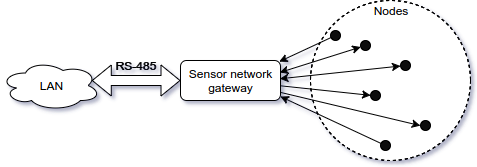
\includegraphics[width=1\textwidth]{01}
    \caption{Blokový diagram funkce gatewaye}
    \label{fig:block diagram of the system}
\end{figure}

Předpokládá se, že koncová zařízení jsou senzory nebo aktuátory napájeny z baterie, tudíž pro jejich dlouhodobou životnost je kladen důraz na nízkou spotřebu vybrané bezdrátové technologie.

Drátová síť RS485, přes kterou gateway komunikuje s PC masterem používá síťový protokol původně navržen pro přístupové systémy. 
Rošiřování vlastností tohoto protokolu by znamenalo mnoho komplikací, cílem je tedy implementace IoT tak, aniž by bylo nutné protokol rozšiřovat.

\section{Přístupové systémy}
Přístupové systémy jsou elektronické systémy řídící skrze síť přístup uživatelů do budov či objektů na základě ověření jejich identity \cite{accessControlSystem_eiprocus}.
V obrázku \ref{fig:Access control system architecture} je znázorněn příklad infrastruktury přístupového systému.

\begin{figure}[!h]
    \centering
    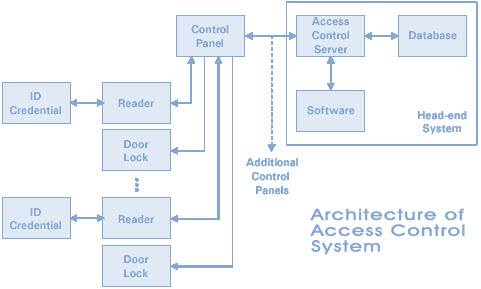
\includegraphics[width=1\textwidth]{Architetcture-of-Access-Control-System}
    \caption{Příklad architektury přístupového systému \cite{accessControlSystem_eiprocus}}
    \label{fig:Access control system architecture}
\end{figure}

todo: popsat jednotlive bloky obrazku

\section{Implementace IoT do přístupového systému firmy IMA}
V použitém systému firmy IMA je control panel nazýván PC Master, který komunikuce s čtečkami proprietárním protokolem přes rozhranní RS485.
Účelem tohoto projektu je tedy nahrad


% todo: 
% - popiste infrastrukturu pristupovych systemu (obrazek a popis jednotlivych bloku), a jednak jejich vyuziti, zda se pouzivaji i na neco jineho - opet clanky, ten obr. 3.1 neni dostatecny pro clanek. Mam na mysli toto:
% https://www.elprocus.com/understanding-about-types-of-access-control-systems/
% https://en.wikipedia.org/wiki/Access_control#Access_control_system_topologies